\documentclass[manuscript, screen, acmsmall]{acmart}
\usepackage[noend]{algorithm2e}
\usepackage{graphicx,balance,multirow,xspace,subcaption,longtable}
\usepackage{tabularx,multirow,booktabs,blindtext}
\usepackage{makecell,amsmath,cleveref,rotating}
\usepackage[font={small}, textfont=md]{caption}
\usepackage[utf8]{inputenc}
\usepackage[draft,inline,nomargin,index]{fixme}
\usepackage{marginnote}
\usepackage[bb=boondox,bbscaled=.95,cal=boondoxo]{mathalfa}
\usepackage{adjustbox}
\usepackage{colortbl}
\usepackage[table,xcdraw]{xcolor}
\usepackage[normalem]{ulem}
\usepackage{wrapfig}
\useunder{\uline}{\ul}{}

\settopmatter{printacmref=false}
\setcopyright{none}

\AtBeginDocument{%
  \providecommand\BibTeX{{%
    Bib\TeX}}}

\PassOptionsToPackage{hyphens}{url}
\usepackage{hyperref}
\usepackage{siunitx}
\usepackage{wasysym} \urlstyle{tt}
\newcolumntype{P}[1]{>{\arraybackslash}p{#1}}
%\newcolumntype{X}[1]{>{\centering\arraybackslash}p{#1}}

\expandafter\def\expandafter\UrlBreaks\expandafter{\UrlBreaks%  save the current one
  \do\a\do\b\do\c\do\d\do\e\do\f\do\g\do\h\do\i\do\j%
  \do\k\do\l\do\m\do\n\do\o\do\p\do\q\do\r\do\s\do\t%
  \do\u\do\v\do\w\do\x\do\y\do\z\do\A\do\B\do\C\do\D%
  \do\E\do\F\do\G\do\H\do\I\do\J\do\K\do\L\do\M\do\N%
  \do\O\do\P\do\Q\do\R\do\S\do\T\do\U\do\V\do\W\do\X%
  \do\Y\do\Z}

\crefformat{section}{\S#2#1#3}
\crefformat{subsection}{\S#2#1#3}
\crefformat{subsubsection}{\S#2#1#3}

\hypersetup{%
  pdftitle={Report for Qualifying Exam},
  pdfauthor={},
  pdfkeywords={},
  bookmarksnumbered,
  pdfstartview={FitH},
  colorlinks,
  citecolor=black,
  filecolor=black,
  linkcolor=black,
  urlcolor=linkColor,
  breaklinks=true,
  hypertexnames=false
}

\clubpenalty=10000
\widowpenalty=10000

\newcommand{\red}[1]{\textcolor{red}{\bf #1}}
\newcommand{\blue}[1]{\textcolor{blue}{\bf #1}}

\newenvironment{packed_itemize}{
\begin{itemize}
  \setlength{\itemsep}{2pt}
  \setlength{\parskip}{0pt}
  \setlength{\parsep}{0pt}
  \setlength{\topsep}{2pt}
}{\end{itemize}}

\newenvironment{packed_enumerate}{
\begin{enumerate}
  \setlength{\itemsep}{2pt}
  \setlength{\parskip}{0pt}
  \setlength{\parsep}{0pt}
  \setlength{\topsep}{2pt}
}{\end{enumerate}}

% \renewcommand{\footnotesize}{\scriptsize}
\newcommand{\etc}{etc.}
\newcommand{\eg}{e.g.,\ }
\newcommand{\etal}{et al.\xspace}
\newcommand{\ie}{i.e.,\ }
\newcommand{\re}{r.e.\ }
\newcommand{\aka}{a.k.a.\ }
\newcommand{\cf}{\emph{cf.\ }}
\newcommand{\note}[1]{\textcolor{blue}{#1}}
\newcommand{\superem}[1]{\underline{\emph{#1}}}
\newcommand{\para}[1]{\vspace{.05in}\noindent\textbf{#1}}
\newcommand{\paraem}[1]{\vspace{.05in}\noindent\emph{#1}}
\newcommand{\yt}{YouTube\xspace}
\newcommand{\X}{$\mathbb{X}$\xspace}
\newcommand\mycommfont[1]{\footnotesize\ttfamily\textcolor{blue}{#1}}

\begin{document}
  \renewcommand\footnotetextcopyrightpermission[1]{} % removes footnote with conference information in first column
  \pagestyle{plain} % removes running headers


  \renewcommand{\sectionautorefname}{\S}
  \renewcommand{\subsectionautorefname}{\S}
  \renewcommand{\subsubsectionautorefname}{\S}

  %! Author = mkeim
%! Date = 7/11/24

% Document
\begin{titlepage}

\newcommand{\HRule}{\rule{\linewidth}{0.5mm}}
\center

\textsc{\LARGE The University of Iowa}\\[1.5cm]

\includegraphics[scale=.1]{figures/iowa}\\[1cm]
\textsc{\Large Report for Qualifying Exam}\\[0.5cm]
%\textsc{\large Ph.D.}\\[0.5cm]
\title {Report for Qualifying Exam}
\HRule \\[0.4cm]
{ \huge \bfseries Shifting Sands: \\Understanding Temporal Context Change}\\[0.4cm]
\HRule \\[1.5cm]


\emph{Author:} \\
Manisha \textsc{Keim} \\
manisha-keim@uiowa.edu \\[0.5cm]

\emph{Advisor:}\\
Rishab \textsc{Nithyanand}\\
rishab-nithyanand@uiowa.edu \\[0.5cm]

Department of Computer Science



{\today}\\[2cm]

\end{titlepage}
  %%%%%%%%%%%%%%%%%%%%%%%%%%% Table of Contents
  \tableofcontents
  \newpage

  %%%%%%%%%%%%%%%%%%%%%%%%%%%% Main document
  %\maketitle
  %\sloppy
  %%! Author = mkeim
%! Date = 7/11/24

% Document
\section{Abstract} \label{sec:abstract}
    In the digital age, online information seekers frequently encounter search results laden with misinformation, biased narratives, and conspiracy theories.
    This exposure can potentially lead users to accept and propagate false information.
    However, this phenomenon is not universal across all search queries.
    Certain searches, known as \textit{data voids} are particularly susceptible to these issues.
    \\
    \textit{Data voids} occur when searching for terms that yield limited, non-existent, or highly problematic relevant information.
    Unlike common searches that produce abundant data, queries falling into data voids may return no results or present irrelevant and often inaccurate information.
    Data voids can be categorized into two main types: newly coined terms with no established information base, and existing terms whose meanings have evolved over time.
    This report focuses on the latter, examining data voids where context drift occurs.
    The following papers has been selected to explore this phenomenon.
    \begin{itemize}
        \item Statistically Significant Detection of Linguistic Change. ACM WWW 2014 \cite{kulkarni2014statisticallysignificantdetectionlinguistic}
        \item Diachronic Word Embeddings Reveal Statistical Laws of Semantic Change. ACL 2016 \cite{hamilton-etal-2016-diachronic}
        \item The Pandemic in Words: Tracking Fast Semantic Changes via a Large-Scale Word Association Task. \cite{10.1162/opmi_a_00081}
    \end{itemize}
  %\newpage
  %! Author = mkeim
%! Date = 7/11/24

\section{Introduction} \label{sec:introduction}
\subsection{What is a Data Void?}
\subsection{Example of a data void?(Migrant Caravan)}
\subsection{Lifecycle of data void (from long tail to spike)}
\subsection{Types of Data Void}
\subsection{Technical Challenge}
analyzing data void involves context drift over historical time. (How context drift happens with data void.)

  \newpage
  %! Author = mkeim
%! Date = 7/11/24

\section{Related Work} \label{sec:relatedwork}
\para{Tracking how word meanings change over time.}
The evolution of word meanings over time has been a subject of significant interest.
Researchers employed a diverse array of methodologies, including \emph{word embeddings} ~\cite{kulkarni2014statisticallysignificantdetectionlinguistic},
\emph{neural language models} ~\cite{kim-etal-2014-temporal}, and \emph{diachronic analysis} ~\cite{hamilton-etal-2016-diachronic, kutuzov-etal-2018-diachronic},
to track and examine semantic shifts across historical periods.
Much of this research utilized the \emph{Google Books Ngram corpus}
~\cite{gulordava-baroni-2011-distributional, kim-etal-2014-temporal, kulkarni2014statisticallysignificantdetectionlinguistic, 10.1007/978-3-319-50496-4_18, hamilton-etal-2016-cultural, hamilton-etal-2016-diachronic, kutuzov-etal-2018-diachronic},
a vast collection spanning from 1900 to 2009,
encompassing over 500 billion books in seven languages.
This dataset provides n-grams with corresponding yearly occurrences and frequencies.

\para{Words can change meaning over time through several linguistic processes.}
Words have the ability to undergo shifts in meaning over the course of time as a result of various linguistic mechanisms,
including but not limited to:
\begin{itemize}
    \item \emph{semantic drift} ~\cite{gulordava-baroni-2011-distributional, kim-etal-2014-temporal, kulkarni2014statisticallysignificantdetectionlinguistic}
    \begin{itemize}
        \item Refers to the evolution of word \underline{\emph{meanings}} over time.
        \item Example: The word `gay' originally meant `happy' or `carefree', but now it predominantly means `homosexual'.
    \end{itemize}
    \item \emph{syntactic alterations} ~\cite{kulkarni2014statisticallysignificantdetectionlinguistic, hamilton-etal-2016-cultural, giulianelli-etal-2020-analysing}
    \begin{packed_itemize}
        \item Syntax focuses on the \underline{\emph{structure}} of language.
        This type of change pertains to modifications in the arrangement of words in sentences.
        \item Example:  The word `apple', which transitioned from being used as a `common noun' (e.g., a fruit) to a `proper noun' (referring to the Apple company) after the company’s rise in the 1980s.
    \end{packed_itemize}
    \item \emph{broadening} ~\cite{kulkarni2014statisticallysignificantdetectionlinguistic, hamilton-etal-2016-cultural, giulianelli-etal-2020-analysing}
        \begin{itemize}
            \item A word’s meaning becomes more general than its earlier meaning, also known as \underline{\emph{generalization.}}
            \item Example: `Holiday' originally meant a religious festival, but now it can refer to any day of celebration or time off.
        \end{itemize}
    \item \emph{narrowing} ~\cite{kulkarni2014statisticallysignificantdetectionlinguistic, giulianelli-etal-2020-analysing}
    \begin{itemize}
            \item A word’s meaning becomes more specific than its earlier meaning, also known as \underline{\emph{specialization}}.
            \item Example: `Literally' used to mean `figuratively' or `symbolically'.
            Now, it is used to emphasize the truthfulness of a statement.
        \end{itemize}
    \item \emph{amelioration}
     \begin{itemize}
            \item A word takes on a more \underline{\emph{positive}} meaning over time.
            \item Example: The word `thrifty' once meant `cheap' but now suggests responsible use of resources.
        \end{itemize}
    \item \emph{pejoration} ~\cite{10.1162/opmi_a_00081, gulordava-baroni-2011-distributional}
        \begin{itemize}
            \item A word takes on a more \underline{\emph{negative}} meaning over time.
            \item Example: The word `awful' meant `full of awe' which transitioned to `terrible' or `appalling'.
        \end{itemize}

\end{itemize}

Hamilton et al.\ (2016) highlighted that \emph{cultural} or \emph{linguistic} factors could have driven these transformations.
Certain studies concentrated on semantic changes, some worked on syntactic changes, ~\cite{kulkarni2014statisticallysignificantdetectionlinguistic, hamilton-etal-2016-cultural, 10.1162/opmi_a_00081}
and others explored the broader evolution that words underwent ~\cite{gulordava-baroni-2011-distributional, kim-etal-2014-temporal, kulkarni2014statisticallysignificantdetectionlinguistic, hamilton-etal-2016-diachronic}.
\Cref{tab:related-work} outlines various types of linguistic changes and the approaches employed to identify them.

\para{Building on the extensive research on \emph{semantic} change.}
Semantic change refers to any change in the meaning(s) of a word over time or acquiring a new sense ~\cite{gulordava-baroni-2011-distributional, 10.1162/opmi_a_00081}.
Kutuzov et al.\ (2018) conducted a survey on semantic shifts, consolidating the existing academic research in this domain.
Their work provides a comprehensive overview of the methodologies and findings related to tracking semantic changes over time using computational techniques.

\begin{table}[]
\centering
\small
\begin{tabular}{@{}llllll@{}}
\toprule
\multicolumn{1}{c}{\textbf{\begin{tabular}[c]{@{}c@{}}Linguistic \\ Change\end{tabular}}} & \multicolumn{1}{c}{\textbf{Approach}}                                              & \multicolumn{1}{c}{\textbf{TCD}} & \multicolumn{3}{c}{\textbf{Example}}                                                                                                                                                                 \\ \cmidrule(l){4-6}
\multicolumn{1}{c}{\textbf{}}                                                             & \multicolumn{1}{c}{\textbf{}}                                              & \multicolumn{1}{c}{\textbf{}}    & \textbf{Word}         & \textbf{Former Usage}                                                                & \textbf{New Usage}                                                                    \\ \midrule
\multicolumn{1}{l}{\textbf{Semantic}}                                                     & \multicolumn{5}{c}{\textbf{FREQUENCY \cite{gulordava-baroni-2011-distributional, kulkarni2014statisticallysignificantdetectionlinguistic, hamilton-etal-2016-diachronic}}}                                             &            &  &                                                                &                                                                 \\ \midrule
\textbf{}                                                                                 & Log Ratio                                                                  & 1960 \& 1990                     & disk                  & -                                                                                    & -                                                                                     \\ \cmidrule(l){2-6}
\textbf{}                                                                                 & \begin{tabular}[c]{@{}l@{}}Word \\ Frequency\end{tabular}                  & 1900--2005                      & bitch                 & female dog                                                                           & slang                                                                                 \\ \cmidrule(l){2-6}

                                                                                          & \multicolumn{5}{c}{\textbf{DISTRIBUTIONAL \cite{gulordava-baroni-2011-distributional, kim-etal-2014-temporal, kulkarni2014statisticallysignificantdetectionlinguistic, 10.1007/978-3-319-50496-4_18, hamilton-etal-2016-diachronic, hamilton-etal-2016-cultural, 10.1162/opmi_a_00081, giulianelli-etal-2020-analysing}}}                                                              &                                  &                       &                                                                                      &                                                                              \\ \cmidrule(l){2-6}
\textbf{}                                                                                 & \begin{tabular}[c]{@{}l@{}}Local Mutual \\ Information\end{tabular}        & 1960 \& 1990                     & sleep                 & deep sleep                                                                           & sleep disorder                                                                        \\ \cmidrule(l){2-6}
\textbf{}                                                                                 & \begin{tabular}[c]{@{}l@{}}Continuous \\ Word \\ Embeddings\end{tabular}   & 1900--2009                      & cell                  & closet, dungeon                                                                      & phone, cordless                                                                       \\ \cmidrule(l){2-6}
\textbf{}                                                                                 & \begin{tabular}[c]{@{}l@{}}Change Point \\ Algorithm\end{tabular}          & 1900--2005                      & gay                   & cheerful, dapper                                                                     & \begin{tabular}[c]{@{}l@{}}lesbian, \\ homosexual\end{tabular}                        \\ \cmidrule(l){2-6}
\textbf{}                                                                                 & Clustering (DBSCAN)                                                        & 1900--2000                      & mouse                 & mice, rat                                                                            & cursor, pointer                                                                       \\ \cmidrule(l){2-6}
\textbf{}                                                                                 & \begin{tabular}[c]{@{}l@{}}Cultural and \\ linguistic Drift\end{tabular}   & 1800--2000                      & virus                 & \begin{tabular}[c]{@{}l@{}}infected with\\  the virus\end{tabular}                   & \begin{tabular}[c]{@{}l@{}}spreading\\  computer virus\end{tabular}                   \\ \cmidrule(l){2-6}
\textbf{}                                                                                 & \begin{tabular}[c]{@{}l@{}}Diachronic \\ Word\\ Embeddings\end{tabular}    & 1800--1999                      & awful                 & full of awe                                                                          & terrible or appalling                                                                 \\ \cmidrule(l){2-6}
\textbf{}                                                                                 & \begin{tabular}[c]{@{}l@{}}Contextual \\ Word \\ Embeddings\end{tabular}                                                                      & 1910 – 2009                      & tenure                & \begin{tabular}[c]{@{}l@{}}short term leases,\\ insecurity of tenure\end{tabular}    & \begin{tabular}[c]{@{}l@{}}tenure of office, \\ employment \\ and tenure\end{tabular} \\ \cmidrule(l){2-6}
\textbf{}                                                                                 & \begin{tabular}[c]{@{}l@{}}Semantic \\ Similarity \\ Analysis\end{tabular} & 2014--2022                      & immunity              & \begin{tabular}[c]{@{}l@{}}politics (‘legislator’,\\ ‘representative’).\end{tabular} & \begin{tabular}[c]{@{}l@{}}health-related \\ (‘prevention’, ‘AIDS’)\end{tabular}      \\ \cmidrule(l){2-6}
                                                                                          & \multicolumn{5}{c}{\textbf{PART OF SPEECH \cite{kulkarni2014statisticallysignificantdetectionlinguistic, hamilton-etal-2016-cultural}}}                                                                       &                                  &                       &                                                                                      &                                                                   \\ \midrule
\textbf{Syntactic}                                                                        & POS Tags                                                                   & 1900--2000                        & windows               & \begin{tabular}[c]{@{}l@{}}doors and \\ windows of a house\end{tabular}              & Microsoft Windows                                                                     \\ \midrule
\textbf{}                                                                                 & \begin{tabular}[c]{@{}l@{}}Mixed-model \\ Regressions\end{tabular}         & 1800--2000                      & actually              & originally, nominally                                                                & presumed, believe\\

\bottomrule
\end{tabular}
%\bottomrule
\caption{\textbf{Comparative Overview of Linguistic Change Detection Approaches.}
This table provides a comprehensive summary of various approaches and contributions to the study of linguistic changes,
    categorizing the type of changes (semantic or syntactic), and detailing the methodologies used, including frequency and distributional approaches.
    It highlights each study’s methods, such as word embeddings, statistical analysis, and clustering, along with the time periods of change detection and examples of changing words.
    The table provides an overview of the advancements and differences in analyzing language evolution,
    capturing the breadth of approaches from traditional frequency counts to modern embedding techniques.}
\label{tab:related-work}
\end{table}

% ------------------------------------------------------------------ SEMANTIC ------------------------------------------------------------------
\begin{itemize}
    \item \textbf{Investigating Semantic Shifts Through Word Contexts.}
    Gulordava and Baroni (2011) detected semantic change by focusing on words used in the 1960s and 1990s.
        They compared the similarity of the surrounding words (words that co-occur with the target word) in these two time periods.
    \begin{itemize}
        \item To assess similarity, the researchers calculated the \emph{Local Mutual Information (LMI)} score between the central word and its surrounding words.
        A low LMI score between the target word and its surrounding words across the two time periods indicated a potential semantic shift.
        \item The study demonstrated that their distributional similarity models were effective in capturing \emph{cultural shifts} in word meaning.
        For example, they found that the word `sleep' acquired more negative connotations related to sleep disorders when comparing its contexts in the 1960s to those in the 1990s.
    \end{itemize}

    \item \para{Tracking Meaning Evolution Through Neural Nets.}
    Kim et al.\ (2014) focused on analyzing how word meanings evolved between 1900 and 2009.
    \begin{itemize}
        \item They developed the first method that employed \emph{prediction-based model} to trace semantic shifts.
        This involved training a model on data from a specific year $y_i$ and then using the resulting word vectors as the starting point for training the model on the next year's data $y_i+1$.
        \item Their method analyzed \emph{global shifts} in a word's vector semantics.
        Additionally, by plotting the time series of a word's distance to its neighboring words in the model's vector space, they visualized the period during which the semantic shift occurred.
        \item They demonstrated this for the word `cell' compared to its early neighbors, `closet' and `dungeon,' and the more recent neighbors, `phone' and `cordless.'
        For `cell,' the identified period of change (1985-2009), which interestingly coincides with the introduction and widespread adoption of cell phones by the public.
    \end{itemize}

    \item \para{Pinpointing Significant Shifts Statistically.}
    Kulkarni et al.\ (2015) proposes a novel computational approach to identify and quantify the semantic and usage changes in words across various media (new products, movies and books).
    \begin{itemize}
        \item Building on the concept of distributed representations proposed by Hinton ~\cite{hinton1986learning}, they map words into a continuous vector space where words with similar meanings are positioned close together.
        \item The approach hinges on constructing \emph{property time series} for each word.
        They propose three methods for constructing these time series (\Cref{sec:paper_hamilton}).:
        \begin{itemize}
            \item \textbf{Frequency:}
            This method analyzes changes in a word's overall frequency of use, assuming a sudden shift in frequency might indicate a semantic shift.
            \item \textbf{Syntactic:}
            This method examines the distribution of a word's part-of-speech tags (e.g., noun, verb) across different time periods, aiming to capture changes in how the word functions grammatically.
            \item \textbf{Distributional:}
            This approach leverages word embeddings which are created for each year, and then alignment is done to represent them in joint embedding space,
            and it's utilized to construct distributional time series for a word's displacement.
        \end{itemize}
        \item Finally, they employed statistically sound \emph{change point detection algorithm} to identify significant moments in these time series, pinpointing the periods where word meaning or usage likely underwent a shift.
        Their results indicated that computational methods for the detection of semantic shifts can be robustly applied to time spans less than a decade.
    \end{itemize}

    \item \para{Word Semantic Modelling of Polysemant.}
        Liao and Cheng (2016) explored the semantic changes of words.
        Their approach built on the understanding that word meaning is closely tied to its context.
        When a word's meaning changes, the surrounding words used with it \emph{(context words)} are likely to change as well.
        They focused on \emph{polysemous} words (words with multiple meanings) and aimed to detect when new meanings emerged.
    \begin{itemize}
        \item They used the \emph{skip-gram architecture with negative sampling} ~\cite{10.5555/2999792.2999959} to obtain word embeddings.
        This technique helped in capturing the contextual meaning of words by representing them in a continuous vector space.
        \item They employed \emph{DBSCAN} to group word embeddings.
        DBSCAN helped in identifying clusters of similar word contexts and distinguishing them from noise, which could indicate semantic changes.
        \item To find similar words, they used a nearest neighbor search method called \emph{Random Project Forest}.
        This method helped in identifying words that are contextually similar to a given word.
        \item Finally, they compared the stability of \emph{similar words} with the stability of their \emph{context words}.
    \end{itemize}

    \item \para{Distinguishing Cultural Shifts from Linguistic Drift.}
    Hamilton et al.\ (2016) addressed the challenge of distinguishing between \emph{cultural shifts} and \emph{linguistic drift}, both of which can contribute to semantic change.
    \begin{itemize}
        \item They proposed two distinct measures based on distributional semantics to distinguish between these two types of semantic change:
        \begin{itemize}
            \item \para{Local Neighborhood Measure:} This measure focused on the closest neighbors (most similar words) in a word's embedding.
            A drastic shift in these nearest neighbors suggests a significant change in core meaning, potentially driven by a \emph{cultural shift}
            (e.g., `gay' changing from carefree to referring to homosexuality).
            \item \para{Global Measure:} This measure considered the overall distribution of a word's surrounding words in a larger context window.
            Gradual changes in this broader distribution are more likely to reflect \emph{linguistic drift}, the natural evolution of language due to regular processes
            (e.g., `promise' expanding from a declaration to also suggesting a likelihood).
        \end{itemize}
        \item Prior research often treated semantic change as a single phenomenon.
        Hamilton et al.\ offered a novel approach by distinguishing between cultural shifts and linguistic drift using their two measures.
    \end{itemize}

    \item \para{Diachronic Analysis on Historical Data: }
    The primary goal of Hamilton et al.\ (2016) is to track semantic changes and understand how the meanings of words shift in different historical contexts.
    \begin{itemize}
        \item They created word embeddings for different time periods using both the PPMI matrix with SVD and the SGNS model.
        These embeddings were generated from historical text corpora to capture the contextual usage of words in each period.
        \item After creating the embeddings, they aligned the embeddings.
        Once the embeddings are aligned, they calculate the \emph{semantic displacement} of a word.
        This essentially measured how much a word's vector representation has moved in the embedding space between two time periods.
        \item The study demonstrates that their method effectively identified semantic change in words and uncovered two statistical `laws' of semantic change:
        \begin{itemize}
            \item \para{Law of Conformity}, which suggests that the rate of semantic change is inversely proportional to a word's frequency.
            High-frequency words tend to change meaning more slowly.
            \item \para{Law of Innovation}, on the other hand, proposes that words with multiple meanings are more likely to undergo semantic transformations over time.
        \end{itemize}
        \item They leveraged the rich information within word embeddings to quantify the degree of semantic change (semantic displacement) and identified potential patterns.
    \end{itemize}

    \item \para{Semantic Shifts with Contextual Embeddings:}
        Giulianelli et al.\ (2020) explored the phenomenon of lexical semantic change using an unsupervised approach using \emph{BERT}.
        \begin{itemize}
            \item They utilized the \emph{BERT} model to generate contextual word embeddings, which captured the meaning of a word based on its surrounding context.
            \item The extracted word usage vectors are then clustered into different \emph{usage types} using the \emph{k-means clustering algorithm}.
            This helped to identify distinct senses or meanings of the words as they appear in various contexts.
            \item They analyzed these clusters for a specific word across different time periods.
            The study proposed three metrics to quantify semantic change:
            \begin{itemize}
                \item \textbf{Entropy Difference (ED)}: Measures the change in uncertainty (entropy) of a word’s usage distribution over time.
                \item \textbf{Jensen-Shannon Divergence (JSD)}: Compares the similarity of word usage distributions across time intervals.
                \item \textbf{Average Pairwise Distance (APD)}: Computes the average distance between word usage vectors from different periods, indicating shifts in word meaning.
            \end{itemize}
            \item The qualitative analysis indicated that the approach could capture various linguistic phenomena, including both synchronic (current usage) and diachronic (historical changes) aspects.
        \end{itemize}

    \item \para{Semantic Similarity:} The impact of significant events like the COVID-19 pandemic on language and semantic change has also been a subject of study.
        Laurino et al.\ (2023) explores tracking fast semantic changes through a large-scale word association task, aiming to understand how the collective mental lexicon evolves in response to such global events.
        Their research highlights the dynamic nature of language and how it incorporates new senses.
        For instance, words like `quarantine', `mask', and `social distancing' took on new and prominent meanings in everyday conversation.
\end{itemize}

% ------------------------------------------------------------------ SYNTACTIC ------------------------------------------------------------------
\para{Linguistic change studies have shifted to include \emph{syntax} alongside semantics.}
The field of linguistic change has traditionally focused on \emph{semantics}.
However, recent studies have begun to explore the role of \emph{syntax} in language evolution as well.
The \emph{syntactic} functionality of a word can evolve by transitioning into a new part-of-speech (POS) category.
Nouns, due to their inherent flexibility in meaning, exhibit a greater tendency to undergo these changes driven by cultural shifts.
While verbs are more likely to participate in gradual semantic changes that follow established linguistic patterns.
\vspace{0mm}
\begin{itemize}
    \item \para{Acquiring a new POS.}
    Kulkarni et al.\ assigned part-of-speech (POS) tags to a large collection of text.
    They calculated the likelihood of a word appearing in specific grammatical contexts over time.
    \begin{itemize}
        \item To quantify temporal change, they compared the probability distributions of POS tags for a particular word across different time periods.
        This essentially measured the divergence between these distributions.
        \item An example they cited was the word `windows'.
        Its POS tag shifted from a common noun (referring to doors and windows of a house) to a proper noun (`Microsoft Windows').
        This highlights how a word's grammatical function can change alongside its meaning.
    \end{itemize}

    \item \para{Capturing Differences Between Nouns and Verbs.}
     Hamilton et al.\ (2016) highlight how \emph{cultural changes}, often influenced by new technologies, are closely tied to transformations within \emph{local neighborhoods}, particularly sensitive to shifts in nouns.
     On the other hand, \emph{linguistic changes} are more associated with \emph{global measures} and are particularly responsive to variations in verbs.
     \begin{itemize}
         \item To validate this hypothesis, the authors employed a statistical technique called a \emph{linear mixed model} where word type (noun or verb) is a fixed effect,
         amount of change measured by each metric (local or global) treated as the dependent variable.
         By analyzing the model's results, they could assess whether there's a significant difference in the way nouns and verbs exhibit change.
         \item The evolution of words like `actually', `must', and `promise' demonstrate these changes.
         For instance, `must' has transitioned from expressing obligation to indicating necessity, showcasing a common pattern seen in modal verbs.
     \end{itemize}
\end{itemize}

% ------------------------------------------------------------------ THREE PAPERS ------------------------------------------------------------------
Several studies from our literature review provide valuable insights for addressing data voids in our analysis.
\begin{itemize}
    \item The first being the work by Kulkarni et al.\ which introduces us to time series construction.
Their distributional methods focuses on finding subtle semantic shits to determine the context where a word in used.
This concept aligns perfectly with our goal of uncovering shifts in word usage when encountering data voids.
    \item Second paper by Hamilton et al.\ introduces us to word emebeddings alignment.
Since we want to compare word vectors from different time periods, vectors should be aligned in same coordinate axes.
After aligning the embeddings for individual time periods, we can use the aligned word vectors to compute the semantic displacement that a word has undergone during a certain time-period.
    \item Third one by Laurino et al.\ investigates the impact of the COVID-19 pandemic on word meaning.
One key finding from their work is that words directly related to the pandemic exhibited a greater difference in semantic similarity between pre-pandemic and pandemic time periods.
This suggests that these words underwent a more significant and rapid semantic shift compared to control words not associated with the pandemic.
They also employ semantic similarity analysis to quantify the shifts in meaning for pandemic-related words and provides evidence that the COVID-19 pandemic acted as a catalyst for rapid semantic change.
\end{itemize}
  \newpage
  %! Author = mkeim
%! Date = 7/18/24

\section{RP1: Statistically Significant Detection of Linguistic Change} \label{sec:paper_kulkarni}
\subsection{Introduction} \label{subsec:kulkarni_introduction}

Kulkarni et al.\ (2015) explores the problem of detecting changes in word usage patterns over time.
They introduce methods to identify words that have undergone significant shifts in \emph{meaning}, usage \emph{frequency}, and \emph{context}.
This is achieved by analyzing historical corpora, which contain vast amounts of text data spanning multiple centuries.
The study utilizes diverse datasets, including Twitter posts, Amazon product reviews, and Google Book Ngrams, to construct time series for individual words.

The research conducted by Kulkarni et al.\ exhibits a compelling alignment with our own research objectives,
specifically focusing on the identification of \emph{data voids} characterized by shifting semantic meanings over time.
Their exploration into these linguistic shifts has revealed interesting insights, such as the evolution of the word `gay,' (\Cref{fig:kulkarni-example})
which transitioned from being cheerful or dapper to signifying homosexual or lesbian aspect around the mid-20th century.

\begin{figure}[htb]
    \centering
    \vspace{-1em}
    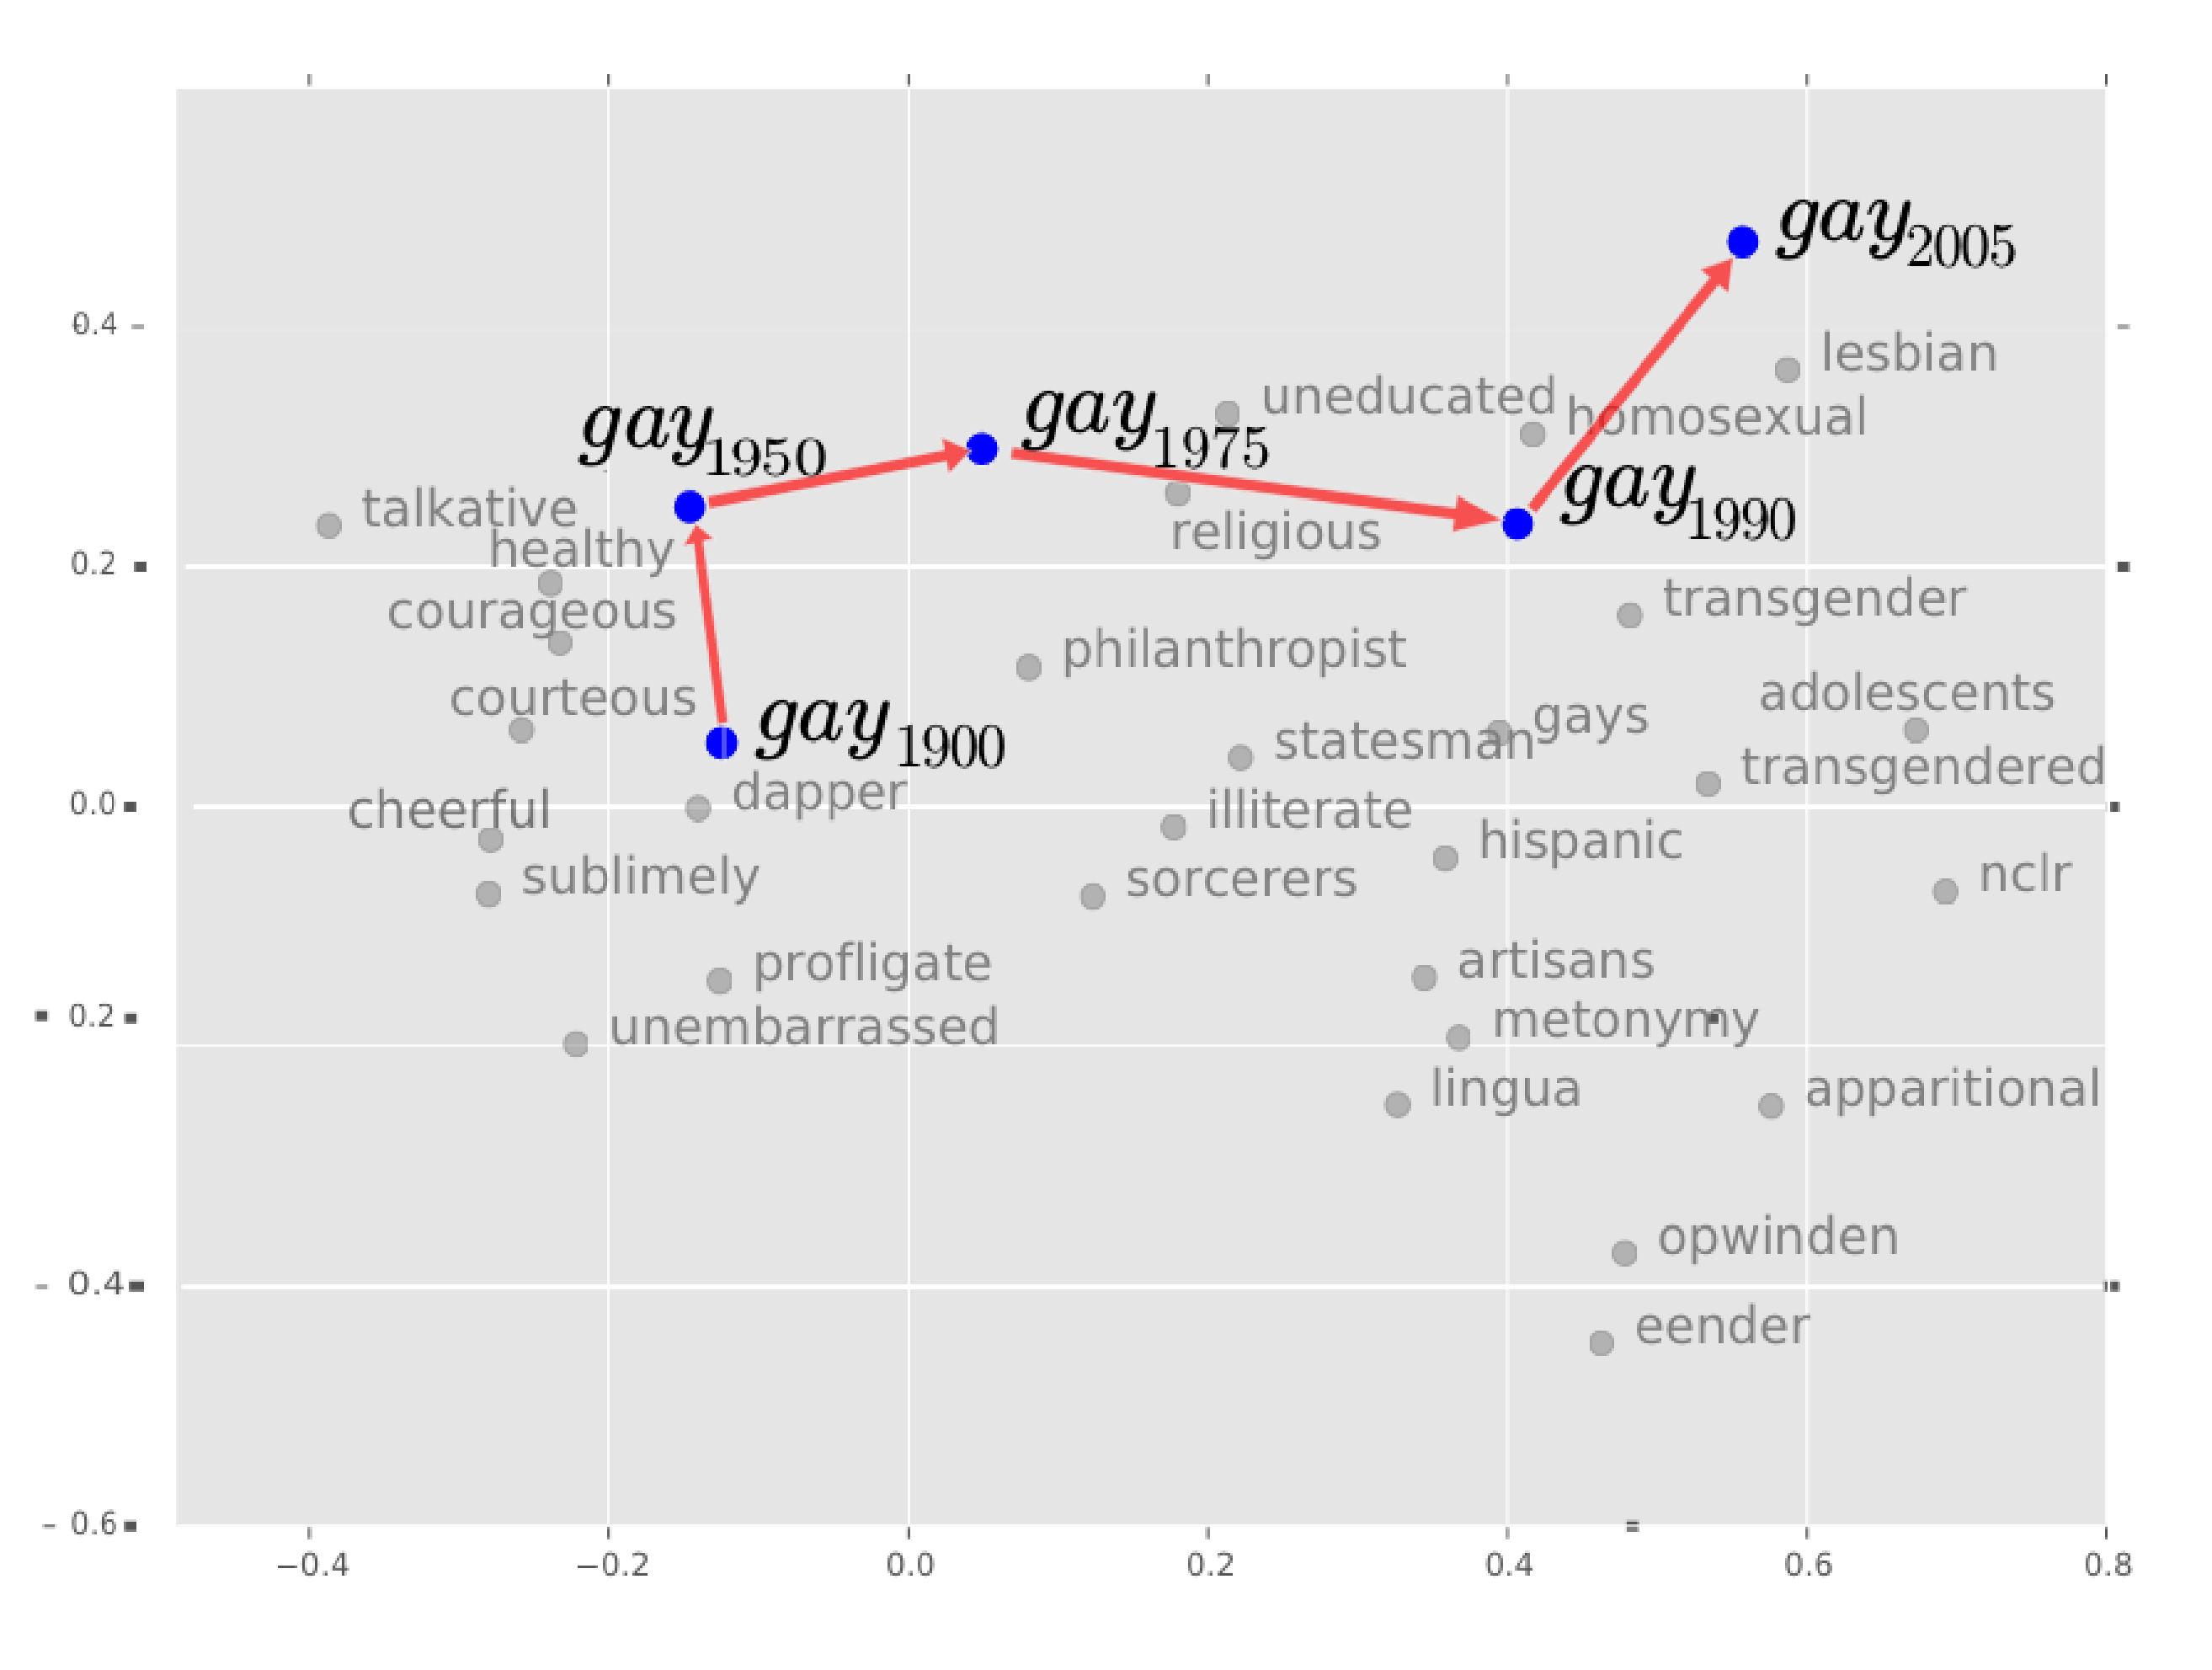
\includegraphics[scale=0.17]{figures/example-gay}
    \vspace*{-0.5cm}
    \caption{Example of word 'gay' undergoing change in meaning over time (taken from \cite{kulkarni2014statisticallysignificantdetectionlinguistic}).}
    \label{fig:kulkarni-example}
\end{figure}

To achieve understanding of this phenomenon, they studied the following research questions.
\begin{itemize}
    \item \para{RQ1.} \emph{What methods can quantify the statistical relevance of observed changes in a word's usage across different time periods?}\\
    Kulkarni et al.’s study uses three technical methods to understand how words change over time: \emph{frequency} analysis, \emph{syntactic} analysis, and \emph{distributional} analysis.
    The frequency method tracks how often words are used, revealing spikes in usage when significant events occur, like how \emph{breaking news} data voids can create a surge in specific keywords.
    The syntactic method looks at changes in the grammatical roles of words, while the distributional method examines word co-occurrence patterns to see how word meanings shift.
    Their approach not only uncovers the dynamic nature of language but also highlights “data voids,” -- areas where terms have \emph{evolved}, become \emph{outdated}, or \emph{fragmented} in meaning.

    \item \para{RQ2.} \emph{Given that a word's usage has changed, how can the precise moment or period of this shift be determined?}\\
    Understanding data voids involves not only recognizing that a change is occurring but also analyzing the specifics of how that change unfolds over time.
    It’s crucial to pinpoint not just the fact that a shift has happened, but also the exact moment when it took place.
    Kulkarni et al.\ tackle this challenge by implementing a \emph{change point detection algorithm} based on the \emph{Mean Shift} model.
    This method determines whether a word has experienced a significant shift and, if so, identifies the precise point at which this change occurred.
\end{itemize}

Next two sections, \Cref{subsec:kulkarni-rq1} and \Cref{subsec:kulkarni-rq2} focuses on the two research questions that this paper is studying, the approach they took to study and their results.

\subsection{What methods can quantify the statistical relevance of observed changes in a word's usage across different time periods?} \label{subsec:kulkarni-rq1}

\para{Overview.}
The challenge is to identify how the meaning of words changes over time.
To address this, they examine a corpus containing data from various domains like books, tweets, and reviews, known as the Temporal Corpus $(C)$ which spans over a time period $(S)$.
This corpus is divided into smaller segments called snapshots $C_t$, each of length $P$.
From these snapshots, a common vocabulary $V$ is created having words which are common across all snapshots.
To analyze changes in these words, a time series $T(w)$ is constructed for each word $w\in V$ (\Cref{fig:kulkarni-overview}).

Kulkarni et al.\ propose several methods to create this time series, aimed at understanding the evolution of words over time.

\begin{figure}[!h]
    \centering
    \vspace{-1em}
    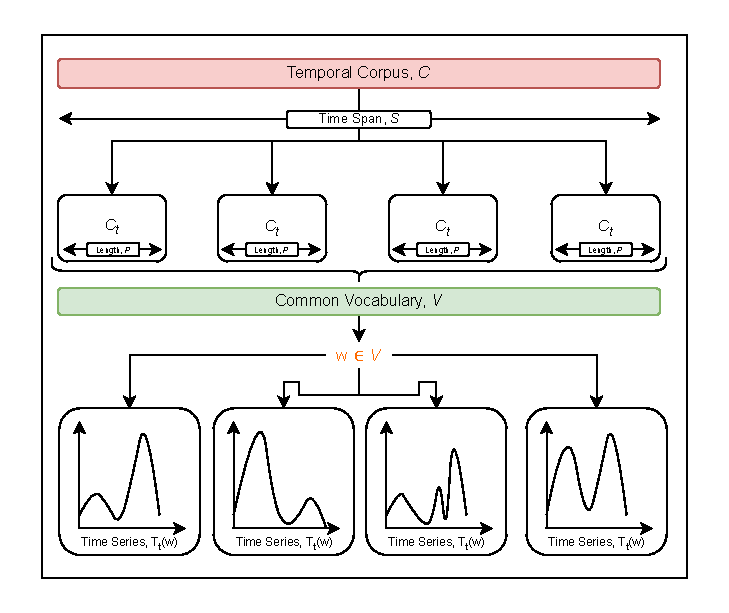
\includegraphics[scale=0.8]{figures/kulkarni_drawio}
    \vspace*{-0.7cm}
    \caption{Overview of time series construction.}
    \label{fig:kulkarni-overview}
\end{figure}

\para{Construction of time series.}
In this paper, three methods are explored for statistically modeling the evolution of words over time:
frequency analysis, part-of-speech tagging, and word co-occurrence to create time series for each word.

\begin{wrapfigure}{r}{0.3\textwidth}
    \centering
    \vspace{-3em}
    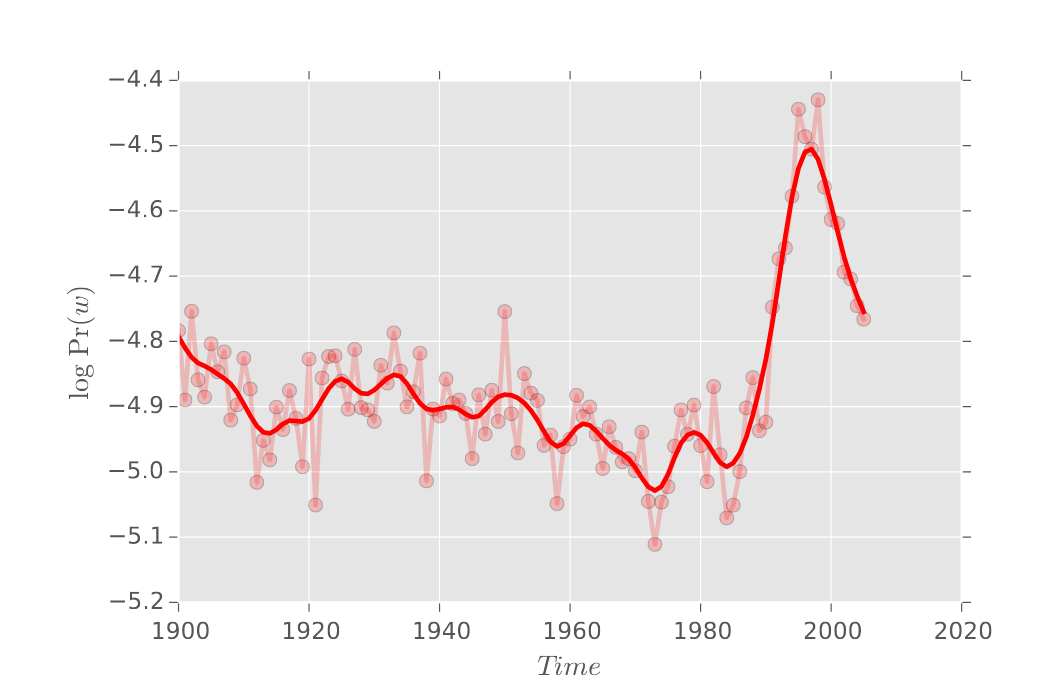
\includegraphics[width=0.35\textwidth]{figures/frequency-gay}
    \vspace*{-1cm}
    \caption{Changes in frequency of 'gay' (taken from \cite{kulkarni2014statisticallysignificantdetectionlinguistic}).}
    \label{fig:example-gay}
\end{wrapfigure}

\para{Frequency method.}
The simplest and most direct method for detecting sudden changes in word usage is by analyzing frequency trends.
This approach examines how often a word is used over a given period, providing insights into shifts in its popularity or relevance.
Changes in frequency can indicate whether a word is gaining new meanings or losing old ones, reflecting broader cultural or societal trends.
For example, the word “gay” in \Cref{fig:example-gay} shows a noticeable spike in usage during the 1980s, signaling a shift in its meaning or cultural relevance.

Tools such as the Google Books Ngram Viewer and Google Trends are used for this purpose, as they provide large datasets and visual representations of word usage across different timeframes.
They calculate the change in probability of a word appearing over time.
\begin{equation}
\mathbf{T_t(w)} = \log \frac{#(w \in C_t)}{|C_t|}
\label{eq:equation}
\end{equation}

\para{Syntactic method.}
Frequency-based metrics, while simple to compute, are susceptible to errors caused by imbalances in the corpus's domain and genre distribution.
Fluctuations in word usage due to temporal events or the popularity of specific entities can obscure genuine shifts in word meaning.
Moreover, a word's grammatical role can evolve over time, such as acquiring a different part of speech category.
To study this, the corpus is annotated with part-of-speech (POS) tags, and the probability distribution of these tags is calculated for each word across different time snapshots.
This approach allows researchers to observe how a word’s syntactic role changes over time.

\para{Distributional method.}
For detecting subtle semantic changes, which are not changed either due to frequency or through change in part of speech,
this method was developed to understand in which context a word is used in and based on that understand the semantic changes.
Distributional methods focusses on creating a semantic space that maps words to continuos vector space, where each word is represented by a vector.
Once they created a temporal word embeddings for each word in each time snapshot, then they track the changes of the represtantations across the embedding space.

The researchers aimed to \emph{learn word embeddings} by training neural language models on a corpus at different time snapshots.
They initialized word vector representations randomly and optimized the model parameters using stochastic gradient descent.
During training, the objective was to maximize the probability of context words appearing around a target word.
After training, word embeddings were normalized by their L2 norm to ensure consistent representation.

The \emph{alignment} process involved aligning word embeddings from different time snapshots into a unified coordinate system to characterize changes between them.
Assumptions were made to aid the alignment process, including the equivalence of spaces under linear transformation and the preservation of local structure of most words over time.
When the alignment model failed to align a word correctly, it indicated a potential linguistic shift, highlighting the importance of accurate alignment for tracking semantic changes over time.
By aligning embedding spaces across various time snapshots into a joint embedding space,
the distributional method constructs a \emph{distributional time series} that captures the semantic evolution of words over time.

The paper shows the evolution of the word `tape' over time.
Initially, the word `tape' referred to an `adhesive tape' but underwent a semantic shift to also mean a `cassette tape'.

\subsection{Takeaways}\label{subsec:takeaways}
For the first research question, Kulkarni et al.\ (2015) explored multiple dimensions of word usage change over time.
To address this, they constructed three types of time series: frequency-based, syntactic, and distributional.

Frequency-based method relies on analyzing the frequency of word usage over time.
It provides immediate insights into trends and spikes in word usage.
However, the frequency method is prone to sampling errors, it may indicate a change in frequency without a significant shift in meaning,
as seen with the word `Hurricane' during events like Hurricane Sandy, where frequency increased but meaning remained stable.
Syntactic-based method analyzes the part of speech (POS) tags of words to detect changes in their syntactic roles over time.
Distributional-based method is based on the fact that words appearing in similar contexts are semantically similar.

Among the three methods employed by Kulkarni et al.\ (2015) for constructing time series,
the distributional time series proved most insightful, as it captures the contextual usage of word.
This approach utilized word embeddings to capture the semantic context of a word within specific time periods.

The syntactic method, while reliable in detecting changes in part-of-speech tags, may overlook significant shifts due to its reliance on linguistic taggers.
At the time of the study, this posed a challenge due to the limitations of tagging accuracy, which has since improved significantly with the advent of more advanced methods for annotating datasets with POS tags.

%back-propogation alogithm
%normalization factor
%negative lof-likelihhod
%stochastic gradient descent
%L2 Norm

\subsection{Given that a word's usage has changed, how can the precise moment or period of this shift be determined?} \label{subsec:kulkarni-rq2}
The authors introduce a method for identifying significant changes in word usage over time using a \emph{change point detection algorithm} based on the \emph{Mean Shift model}.
The process begins by constructing time series data for each word in the corpus—whether using frequency-based, syntactic, or distributional methods.
The next step is to determine if the word has experienced a significant change.
If a significant shift is detected, the algorithm then identifies and returns the \emph{estimated change point (ECP)}, which marks the time when this change occurred.

Since language exhibits a stochastic drift.
In this context, `stochastic' refers to the randomness or probabilistic nature of the training process,
where the models are trained on the same dataset but may produce different results each time due to this randomness.
To resolve this, time series was normalized for each word by transforming the time series into a \emph{Z-score series}.

The Mean Shift model is then applied, which involves calculating the mean of the time series data before and after each potential change point.
By comparing these means, the algorithm determines if a statistically significant change has occurred at any given point in time.

%\begin{figure}[htb]
%    \centering
%    \vspace{-1em}
%    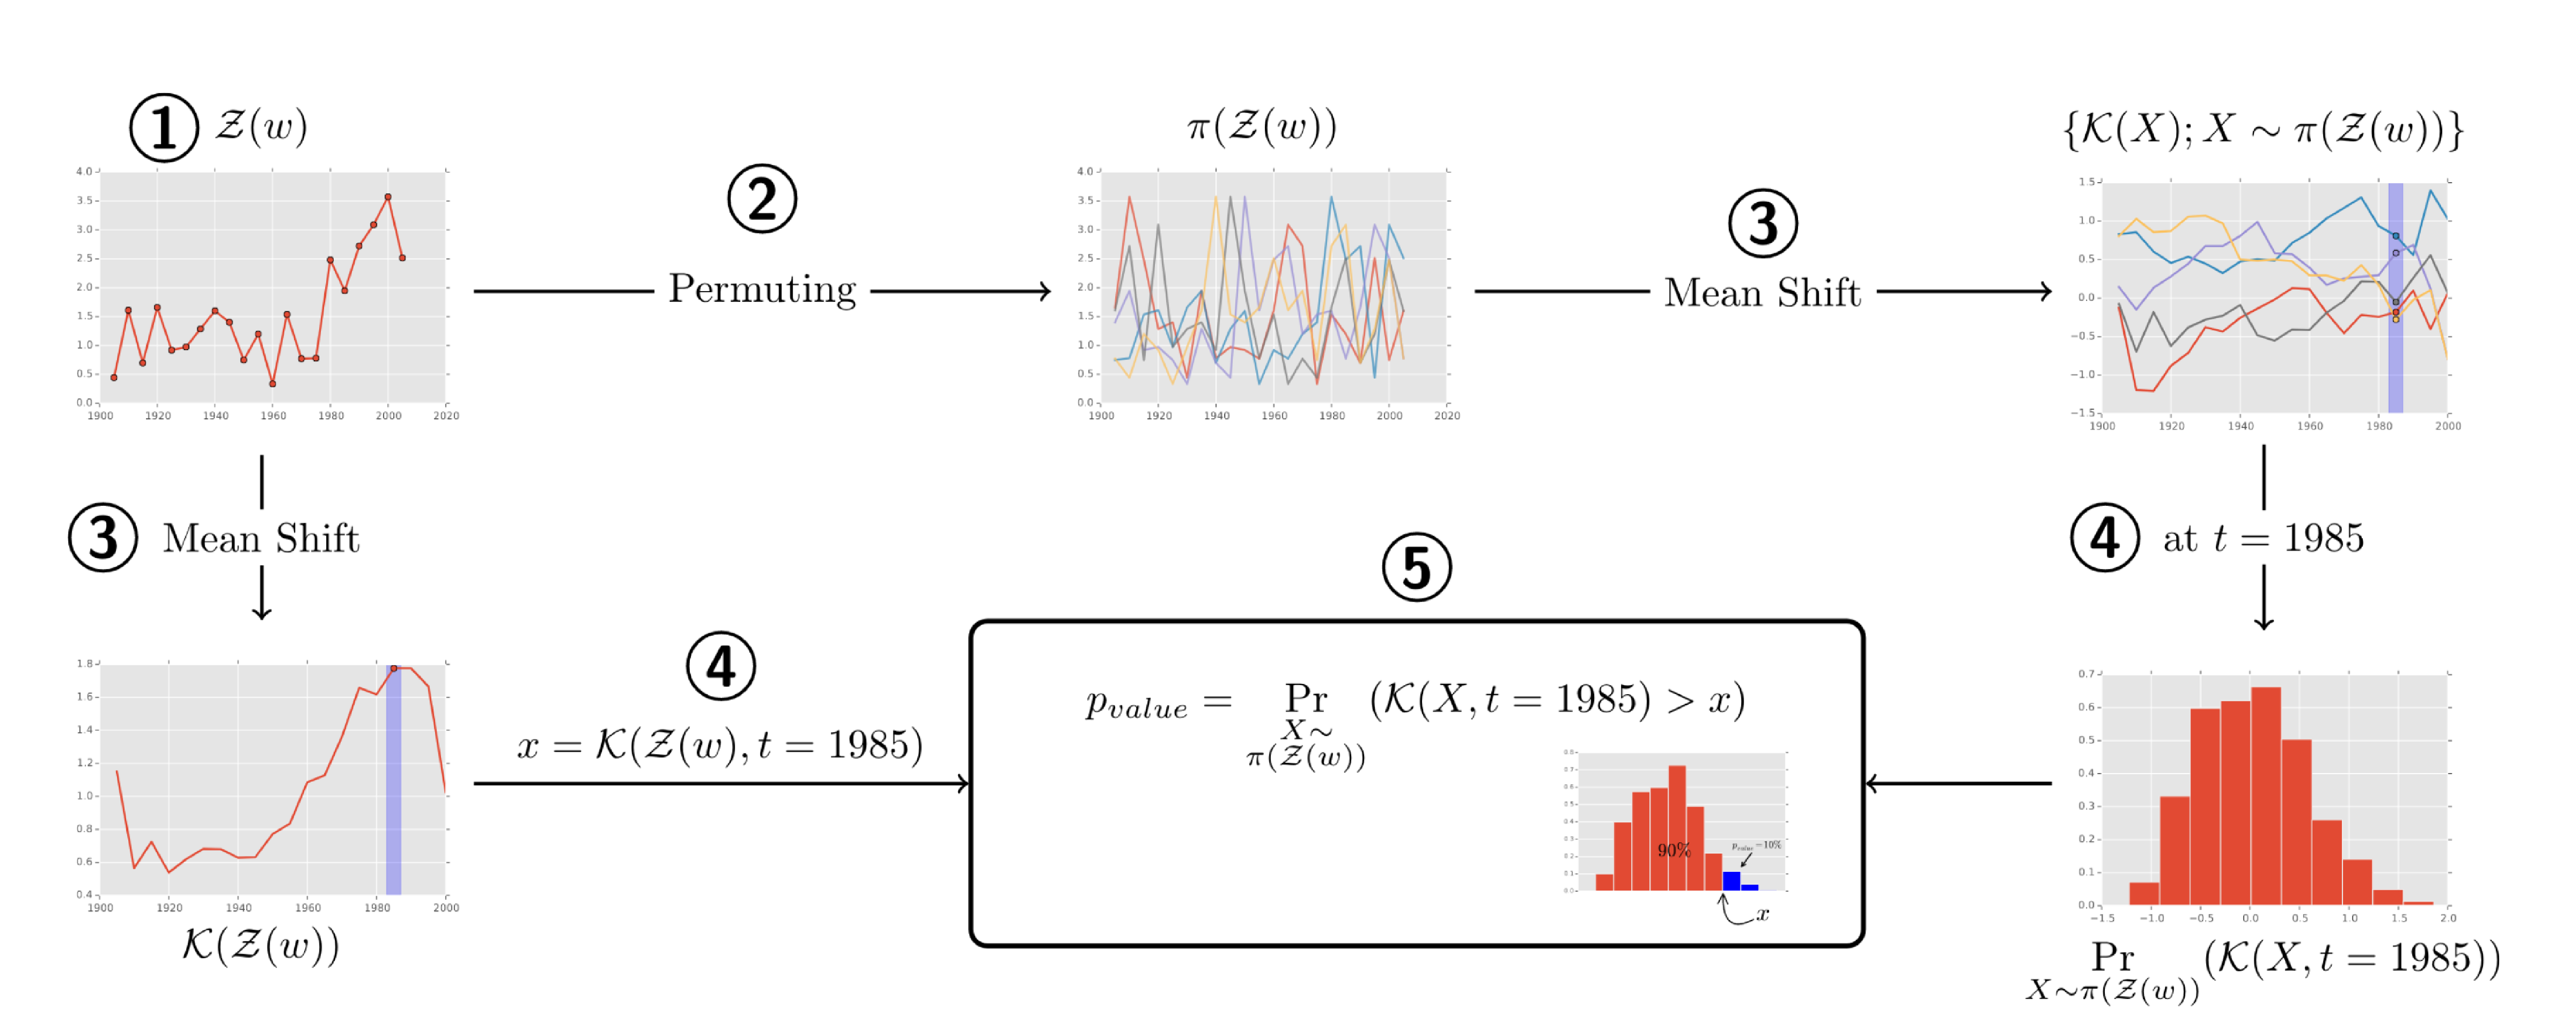
\includegraphics[scale=0.17]{figures/changepoint}
%    \vspace*{-0.5cm}
%    \caption{Change Point Algorithm (taken from \cite{kulkarni2014statisticallysignificantdetectionlinguistic}).}
%    \label{fig:kulkarni-changepoint}
%\end{figure}

\para{Change point algorithm.}
After constructing time series data for each word in the corpus—whether using frequency-based, syntactic, or distributional methods (\Cref{subsec:constructing-word-embeddings}), the first step is to normalize the time series data for the word $w$.
After normalization, the algorithm computes a mean shift series, denoted as $K(Z(w))$.
The \emph{mean shift} is defined as the difference in the mean of a time series at different time points.
The algorithm calculates this shift by segmenting the time series around a pivot point, denoted as time point $j$, and comparing the means of the segments before and after this point.
To assess the significance of the computed mean shifts, the algorithm employs a \emph{bootstrapping} method.
The algorithm uses bootstrap sampling to ensure that the detected change point is not just due to random noise.
It generates multiple synthetic time series by randomly resampling the original time series, denoted as $BS$.
These resampled sets serve as a reference to evaluate whether the detected shifts in the real data are significant or not.
This is done by repeatedly drawing samples from the normalized data $Z(w)$ until the number of samples equals $B$, which is predefined.
For each sample, the algorithm calculates a p-value for each time point $i$.
This p-value indicates how likely it is that the observed change at that time point is significant.
The algorithm identifies potential change points by looking for times $j$ where the Z-Score $Z_j(w)$ is greater than or equal to the threshold $\gamma$.
It then checks the p-values for these change points and selects the one with the smallest p-value, indicating the most significant change.
The algorithm returns the p-value and the estimated change point (ECP).
This information helps understand exactly when the meaning or usage of the word has shifted over time.
%\Cref{fig:kulkarni-changepoint} illustrates the important aspects of the algorithm.

\subsection{Takeaways}\label{subsec:takeaways2}
The change point detection algorithm (\Cref{subsec:kulkarni-rq2}) presented in the paper detects significant linguistic shifts over time by analyzing word time series data.
To detect changes, they first convert these time series into Z-score series, which normalize the data and make it easier to identify shifts.
The Mean Shift model is then applied, which involves calculating the mean of the time series data before and after each potential change point.
By comparing these means, the algorithm determines if a statistically significant change has occurred at any given point in time.

The paper illustrates this with the example of the word `tape,' which transitioned from meaning adhesive tape to cassette tape, with the change detected in the \emph{1970s}.
Similarly, the word `apple' shifted from being used primarily as a common noun to a proper noun associated with Apple Inc., with this change occurring around \emph{1984}.

These examples illustrate the algorithm’s capability to pinpoint when a word’s usage and meaning undergo significant shifts.
The paper emphasizes the importance of analyzing these changes to understand linguistic evolution better.

\subsection{Results} \label{subsec:kulkarni-results}

\para{Time series analysis \& historical analysis.}
The results presented in Kulkarni et al.\ (2015) illustrate how words acquire new meanings and how these meanings change over time through time series and historical analysis.

\para{Frequency method.}
For words like `transmitted,' `bitch,' `sex,' and `her,' the frequency and distributional methods reveal significant insights.
For example, the sharp increase in the frequency of the word `her' around the 1960s can be attributed to the concurrent rise of the feminist movement.
However, the frequency method can produce many false positives due to the temporary popularity of specific social and political events.

\begin{table}[tbh]
\begin{tabular}{@{}lllll@{}}
\toprule
\textbf{Method}         & \textbf{Examples}                              &  &  &  \\ \midrule
\textbf{Frequency}      & transmistted, bitch, sex, her                  &  &  &  \\
\textbf{Syntactic}      & apple, hug, sink, click, handle, windows, bush &  &  &  \\
\textbf{Distributional} & diet, tape, plastic                            &  &  &  \\ \bottomrule
\end{tabular}
\caption{Time Series Analysis}
\label{tab:time-series-examples}
\end{table}
\raggedbottom

\para{Syntactic method.}
The syntactic method uniquely detected the word `apple,' which saw its most frequent part of speech tag shift significantly from `Noun' to `Proper Noun.'
This method has a low false positive rate but suffers from a high false negative rate, as evidenced by its detection of only two words in the study.

\para{Distributional method.}
For words like `diet,' `tape,' and `plastic,' the distributional method sheds light on significant changes in their usage.
The popularity of dieting books, starting with the bestseller `Dr. Atkins’ Diet Revolution' by Robert C. Atkins in 1972, shifted the meaning of `diet' from simply referring to the food consumed to a lifestyle of food consumption behavior.

These findings demonstrate the nuanced ways in which word meanings evolve and the strengths and limitations of different methods in detecting these changes.
\Cref{tab:time-series-examples} shows all the examples that the paper have shown for different methods.
While frequency and distributional methods can highlight shifts in usage, they are prone to false positives.
The syntactic method, though precise, may miss many significant changes.
Therefore, a combined approach utilizing all methods may offer the most comprehensive insights into linguistic evolution

\para{Cross domain analysis.}
The study extends its analysis to datasets like Amazon Reviews and Twitter, which cover much shorter time scales compared to the Google Books Ngram Corpus.
This cross-domain analysis explores the impact of applying the distributional method on these more temporally constrained datasets.
\Cref{tab:sources-examples} presents words that exhibit semantic change across various datasets.

\begin{table}[tbh]
\begin{tabular}{@{}lllll@{}}
\toprule
\textbf{Dataset Source} & \textbf{Examples}                     &  &  &  \\ \midrule
\textbf{Amazon Reviews} & streaming, ray, combo, rays, twilight &  &  &  \\
\textbf{Twitter Tweets} & candy, myster, rally, sandy           &  &  &  \\ \bottomrule
\end{tabular}
\caption{Cross Domain Analysis}
\label{tab:sources-examples}
\end{table}
\raggedbottom

In the Twitter dataset, the word `sandy' acquired a new sense following Hurricane Sandy hitting the East Coast of the USA\@.
Similarly, the analysis on Amazon Reviews revealed changes in words associated with new products and technology trends.

These words demonstrate the method’s ability to capture emerging usages and meanings.
The example of `sandy' highlights how a natural disaster can influence linguistic shifts, with the word gaining a new context and meaning after the hurricane event.

These examples demonstrate that the method can effectively detect the introduction of new products, movies, and books, showcasing its adaptability to different domains and time scales.
This cross-domain capability is particularly valuable for identifying and understanding contemporary linguistic changes in rapidly evolving contexts like social media and online reviews.

\subsection{Takeaways} \label{subsec:kulkarni-takeaways}
The paper by Kulkarni et al.\ (2015) presents an innovative approach to detecting significant linguistic changes over time using statistical methods and word embeddings.
The goal behind their work is to systematically track and analyze how words evolve in meaning and usage across different temporal contexts.
They construct time series for each word using three distinct methods:
frequency, which captures the prevalence of word usage over time;
syntactic, which examines shifts in part-of-speech tags;
and distributional, which looks at changes in word co-occurrence patterns.
They also employ a change point detection algorithm which identifies estimated change points, where significant linguistic shifts occur.
Their analysis spans various datasets, including Google Books Ngram Viewer, Amazon Reviews, and Twitter,
demonstrating the method’s adaptability and effectiveness in detecting both gradual and abrupt changes in word meanings across different domains and time scales.
  \newpage
  %! Author = mkeim
%! Date = 7/18/24

\section{RP2. Diachronic Word Embeddings Reveal Statistical Laws of Semantic Change} \label{sec:paper_hamilton}
\subsection{Introduction}\label{subsec:hamilton_introduction}
Hamilton et al.\ (2016) explores the dynamic nature of language by analyzing how word meanings evolve over time.
Using \emph{diachronic} (historical) word embeddings, a technique that maps words into vector spaces based on historical corpora, the study uncovers patterns and laws governing semantic shifts.
Their approach provides a quantitative framework to examine how words change meaning, influenced by cultural, and linguistic factors.

The pace at which words undergo semantic change differs, with some words changing meaning more frequently compared to others.
For example, the word `cat' has remained relatively stable in its meaning, while `cast' has evolved to have multiple meanings ~\cite{hamilton-etal-2016-diachronic}.

There are several hypotheses about the patterns in semantic change, including the increasing subjectification of meaning or the grammaticalization.
This paper, however, focuses on following two specific questions about semantic change:
\begin{itemize}
    \item \para{RQ1.} \emph{What role does word frequency play in the evolution of word meanings?}\\
    Frequency is a significant factor in linguistic changes, with high-frequency words often changing faster, while low-frequency words tend to be more resistant to change.
    The connection between word frequency and semantic change is a key unanswered question in the field of linguistics.
    The authors introduce the \textbf{law of conformity} to address this gap, demonstrating that frequent words change more slowly, and it clarifies the role of frequency in semantic change.

    \item \para{RQ2.} \emph{How does polysemy relate to semantic change?}\\
    Another unresolved question in linguistics is the relationship between semantic change and polysemy.
    Polysemous words, which have multiple meanings, appear in a variety of contexts.
    It remains unclear whether the diverse contextual use of these words makes them more or less prone to undergoing semantic change.
    The authors propose the \textbf{law of innovation}, which demonstrates that polysemous words are more likely to experience faster semantic changes.
    If a word has multiple meanings, it is more likely to lead to semantic change, especially in the case of rare senses.
\end{itemize}

In our work on data voids, we have recognized that word frequency significantly impacts their identification.
For instance, the term `sandy' saw a spike in usage during the Hurricane Sandy event (\Cref{subsec:kulkarni-results}).
Similarly, terms associated with political agendas also experience increased usage during relevant events.
This paper provides insights into how frequency influences the evolution of word meanings.

Additionally, our study identifies data voids involving polysemous terms, such as `migrant caravan.'
This term began to change in meaning when FOX News used it to describe people moving from the Mexico border towards the US, and it continued to evolve with new groups of migrants.
Understanding these kinds of data voids is crucial, and this paper helps us identify subtle semantic changes in words with multiple meanings,
enhancing our understanding of how these changes relate to frequency and context.

The paper aims to develop a robust methodology for quantifying semantic change using word embeddings and comparing different approaches to analyzing semantic change.
This methodology is then applied in a large-scale cross-linguistic analysis spanning 200 years and four languages
(English, German, French, and Chinese) to propose the above two statistical laws relating frequency and polysemy to semantic change.

\subsection{Constructing Word Embeddings}\label{subsec:constructing-word-embeddings}
The authors employ three methods to construct word embeddings for different time periods.
Initially, they create embeddings for each distinct period and then align these embeddings over time to maintain consistency.
To quantify semantic change, they use various metrics.
Specifically, they utilize Singular Value Decomposition (SVD), Positive Pointwise Mutual Information (PPMI), and Skip-Gram with Negative Sampling (SGNS).
These distributional techniques represent each word by a vector that encapsulates information about the word’s co-occurrence statistics.

\para{Positive Pointwise Mutual Information (PPMI). }
PPMI is a statistical measure used to quantify the association between a word and its context within a corpus.
In the paper, it is used to create word embeddings by capturing the strength of association between words and their co-occurring contexts over time.

First, a co-occurrence matrix is built, where each entry represents the frequency with which a word (target) and its context (typically a window of neighboring words) appear together in the corpus.
The \emph{joint probability} of a target word $w_i$ and a context word $c_j$ is calculated by dividing the co-occurrence frequency of $w_i$ and $c_j$ by the total number of word pairs in the corpus.
The \emph{marginal probability} of the target word $w_i$ and the context word $c_j$ are calculated based on the total occurrences of each word in the corpus.
The Positive Pointwise Mutual Information (PPMI) between the target word $w_i$ and the context word $c_j$ is calculated using the formula:
\begin{equation}
\mathbf{M}^{\text{PPMI}}_{i,j} = \max \left\{ \log \left( \frac{\hat{p}(w_i, c_j)}{\hat{p}(w_i) \hat{p}(c_j)} \right) - \alpha, 0 \right\},
\label{eq:ppmi}
\end{equation}

where:
\begin{itemize}
\item $\hat{p}(w_i, c_j)$ is the \emph{joint probability} of the target word $w_i$ and the context word $c_j$ occurring together.
\item $\hat{p}(w_i)$ and $\hat{p}(c_j)$ are the \emph{marginal probabilities} of the target word $w_i$ and the context word $c_j$, respectively.
\item $\alpha > 0$ is a positive constant used to smooth the values and prevent extreme positive values in the PPMI calculation.
\end{itemize}

This formula refines the PPMI measure by incorporating $\alpha$ to adjust the log probability ratio.
The inclusion of $\alpha$ helps manage the sparseness of the data and the impact of low-frequency events, making the measure more robust and stable.

\para{Singular Value Decomposition (SVD). }
SVD is a mathematical technique that factorizes a matrix into three other matrices, revealing important features of the original matrix.
In the context of word embeddings, SVD helps to reduce the dimensionality of the data while preserving the essential structure and patterns in word co-occurrences.
SVD decomposes the co-occurrence matrix into three matrices in the following manner:
\begin{equation}
\mathbf{w}_i^{\text{SVD}} = (\mathbf{U} \Sigma^\gamma)_i,
\label{eq:svd}
\end{equation}

where:
\begin{itemize}
    \item $\mathbf{w}_i^{\text{SVD}}$ is the vector representation of the word $w_i$ in the SVD-based embedding space.
    \item $\mathbf{U}$ is the matrix of left singular vectors obtained from the decomposition of the co-occurrence matrix.
    \item $\Sigma$ is the diagonal matrix of singular values.
    \item $\gamma$ is a parameter that scales the singular values, allowing for tuning the influence of the different components.
\end{itemize}

In this formula, the word vector $\mathbf{w}_i^{\text{SVD}}$ is derived by scaling the singular values in $\Sigma$ by $\gamma$ and then multiplying by the corresponding vectors in $\mathbf{U}$.
This approach provides a flexible way to adjust the contribution of the components to the final word embeddings.

\para{Skip-Gram with Negative Sampling (SGNS). }
SGNS is a technique used to learn high-quality word vectors by training on large corpora.
The primary goal of SGNS is to learn word embeddings such that words that appear in similar contexts have similar vector representations.
For a given target word $w$ and a context word $c$, the model tries to maximize the probability $P(c|w)$
\begin{equation}
\hat{p}(c_i \mid w_i) \propto \exp(\mathbf{w}_i^{\text{SGNS}} \cdot \mathbf{c}_j^{\text{SGNS}}),
\label{eq:sgns}
\end{equation}

where:
\begin{itemize}
    \item $\hat{p}(c_i \mid w_i)$ is the estimated probability of a context word $c_i$ given a target word $w_i$.
    \item $\mathbf{w}_i^{\text{SGNS}}$ is the vector representation of the target word $w_i$ in the SGNS embedding space.
    \item $\mathbf{c}_j^{\text{SGNS}}$ is the vector representation of the context word $c_j$ in the SGNS embedding space.
\end{itemize}

The probability $\hat{p}(c_i \mid w_i)$ that a word $c_i$ is a context word of $w_i$ is proportional to the exponential of the dot product of their corresponding vector representations.
The dot product $\mathbf{w}_i^{\text{SGNS}} \cdot \mathbf{c}_j^{\text{SGNS}}$ measures the similarity between the target word and the context word in the vector space.
A higher dot product indicates that the words are more likely to co-occur, leading to a higher estimated probability.

The model uses this probability estimation to distinguish true word-context pairs from randomly sampled negative pairs.
The training objective is to maximize the probability of observed (target, context) pairs and minimize the probability of randomly sampled pairs, thereby learning embeddings that reflect the semantic relationships between words.

\para{Aligning Embeddings.}
Words that have similar meanings across different time periods should ideally have similar embeddings.
Alignment ensures that the embeddings from different periods are comparable, making it possible to observe how a word’s meaning shifts over time.

This alignment process involves finding the best way to rotate and transform the embeddings from one time period so that they closely match the embeddings from the next period.
This is done by finding an orthogonal transformation matrix (let’s call it $\mathbf{R}^{(t)}$) that minimizes the difference between the embeddings from two consecutive time periods.
The transformation ensures that distances and angles between word vectors (which represent their meanings) are preserved, allowing for an accurate comparison.
By aligning the embeddings, the authors could measure the semantic displacement of words—how much the meaning of a word has shifted from one time period to another.

\subsection{Takeaways}\label{subsec:hamilton_takeaways1}
The authors created three types of word embeddings using PPMI, SVD, and SGNS, each capturing different information.
PPMI measures how closely related two words are, resulting in sparse, high-dimensional vectors.
SVD simplifies this information by reducing the dimensionality of the PPMI matrix into dense, low-dimensional vectors.
Lastly, SGNS learns embeddings by predicting surrounding words in a given context, uncovering deeper semantic and contextual nuances that the other methods may not capture.
Additionally, they employed alignment technique to align word embeddings across different time periods, ensuring consistency and enabling the analysis of semantic shifts over time.

\subsection{Measuring Semantic Change}\label{subsec:measuring-semantic-change}
Once the embeddings are aligned, following methods are performed to quantify how much the meaning of word changes over time.
\begin{itemize}
    \item \para{Pair-wise similarity time-series}
        This method measures changes in the similarity between pairs of words over different time periods using cosine similarity.
        \begin{equation}
            s^{(t)}(w_i, w_j) = \text{cos-sim}(w_i^{(t)}, w_j^{(t)})
            \label{eq:equation2}
        \end{equation}
        The Spearman correlation $(\rho)$ is employed to measure the relationship between the similarity scores of word pairs and time.
        This non-parametric method assesses whether the similarity series shows a significant increase or decrease over time, which helps us identify specific linguistic or cultural shifts.

    \item \para{Measuring semantic displacement}
        This method quantifies how much a word's meaning has changed by calculating the displacement of its vector representation across different time points.
        They use the aligned word vectors to compute the \emph{semantic displacement} that a word has undergone during a certain time-period.
        It is measured by calculating the distance between the vector representations of a word in different time periods.
        For a given word $w$, if $\mathbf{w}^{(t1)}$ and $\mathbf{w}^{(t2)}$ are its embeddings in two time periods $t1$ and $t2$, respectively, then the semantic displacement $\Delta$ is computed as:
        \begin{equation}
            \Delta(w) = \text{cos-dist}(\mathbf{w}^{(t1)}, \mathbf{w}^{(t2)}).\label{eq:equation3}
        \end{equation}
\end{itemize}

\subsection{Evaluation \& Results}\label{subsec:evaluation&results}
In this paper, the authors compared different word embedding approaches — PPMI, SVD, and SGNS (\Cref{subsec:constructing-word-embeddings}) by evaluating them
on \emph{synchronic accuracy} (similarity within time-period) and \emph{diachronic validity} (semantic changes over time).

%\begin{figure}[htb]
%    \centering
%    \vspace{-1em}
%    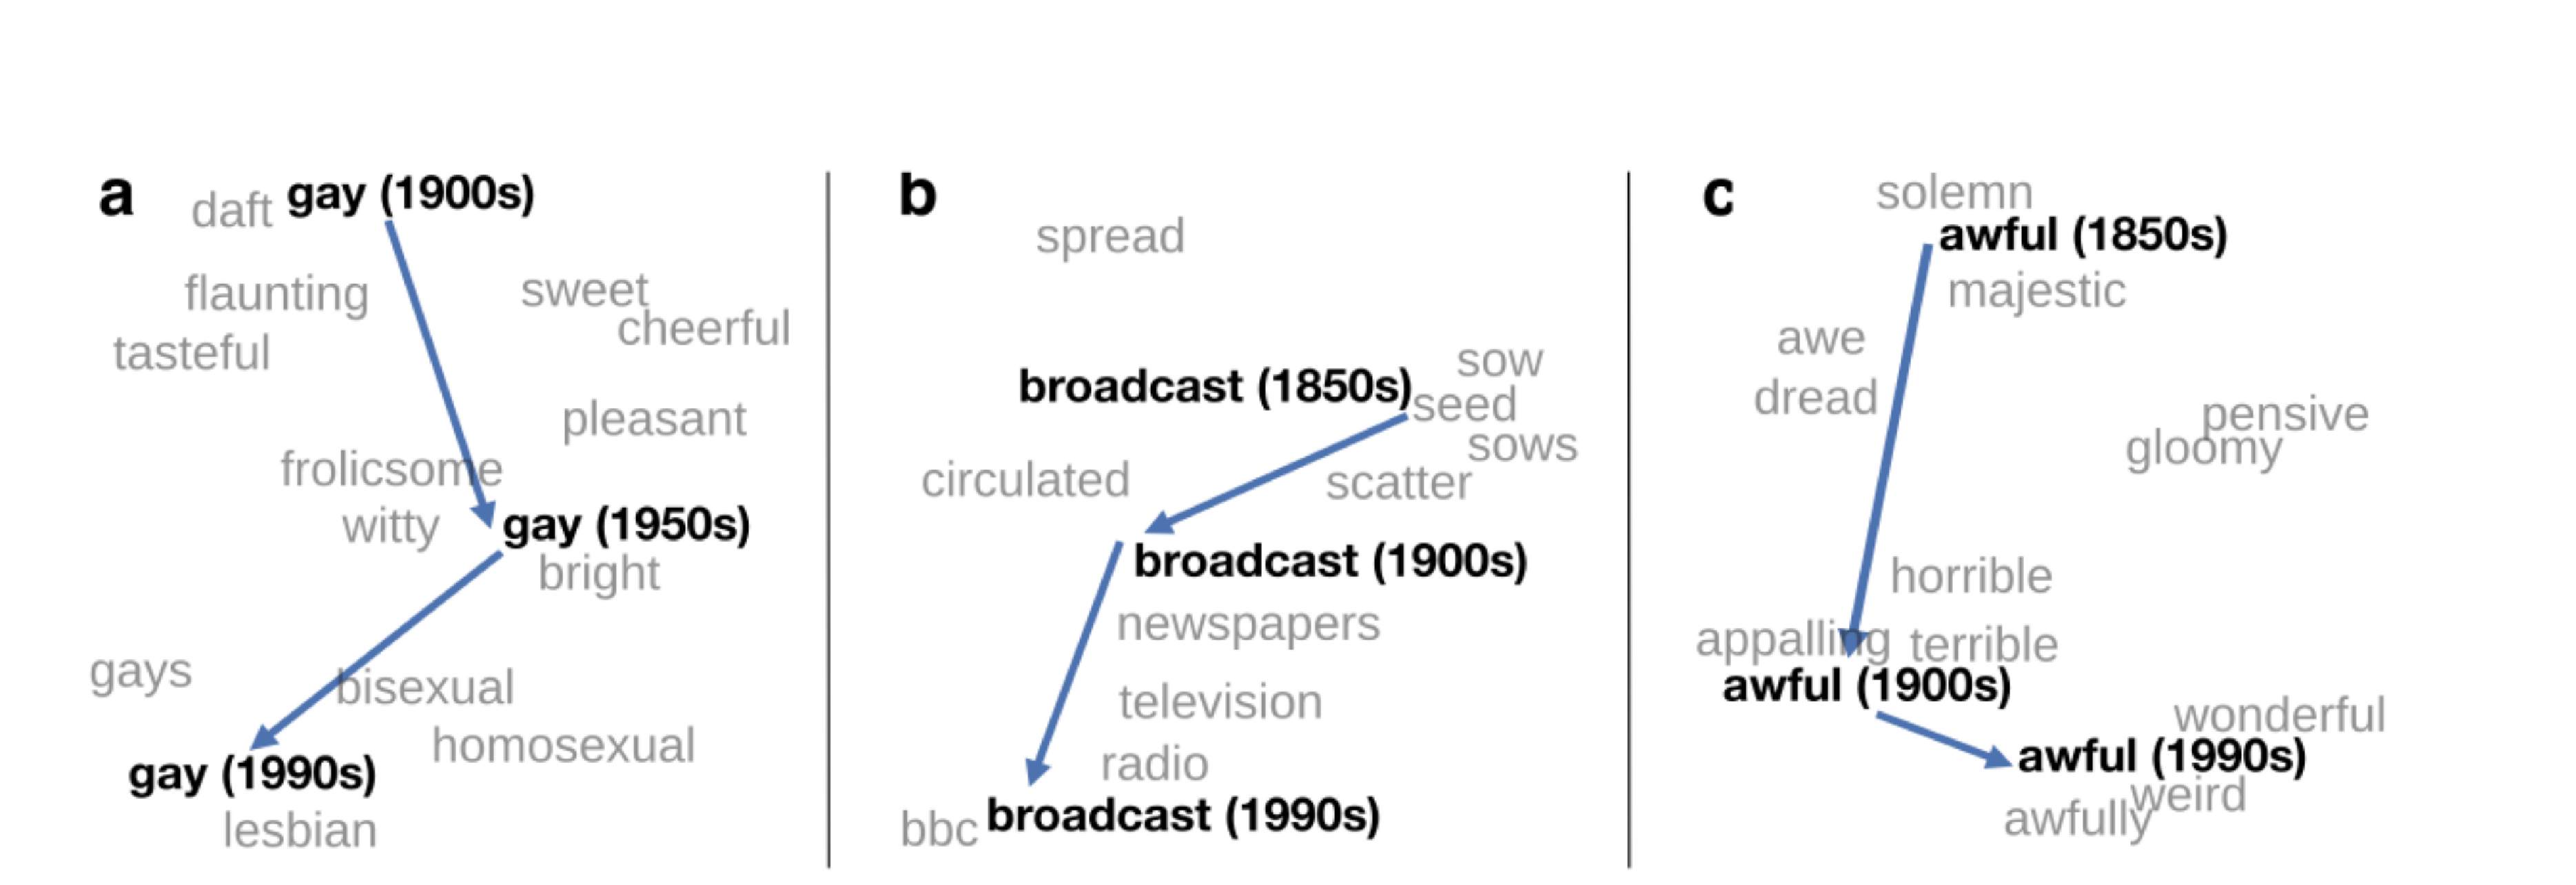
\includegraphics[scale=0.17]{figures/hamilton}
%    \vspace*{-0.5cm}
%    \caption{Example of word 'gay' undergoing change in meaning over time (taken from \cite{hamilton-etal-2016-diachronic}).}
%    \label{fig:hamilton-example}
%\end{figure}

\para{Synchronic Accuracy.}
Synchronic accuracy refers to the accuracy with which word embeddings capture the semantic relationships and meanings of words at a \emph{specific point in time}.
It assesses how well the models represent the semantic relationships among words in a given time period.
SVD performed best here followed by PPMI and SGNS\@.

\para{Diachronic Validity.}
Diachronic validity evaluates how effectively the methods can detect and quantify changes in \emph{meaning over time}.
The authors evaluate the diachronic validity of their methods through two main tasks:

\begin{figure}[tbh]
    \centering
    \vspace{-1em}
    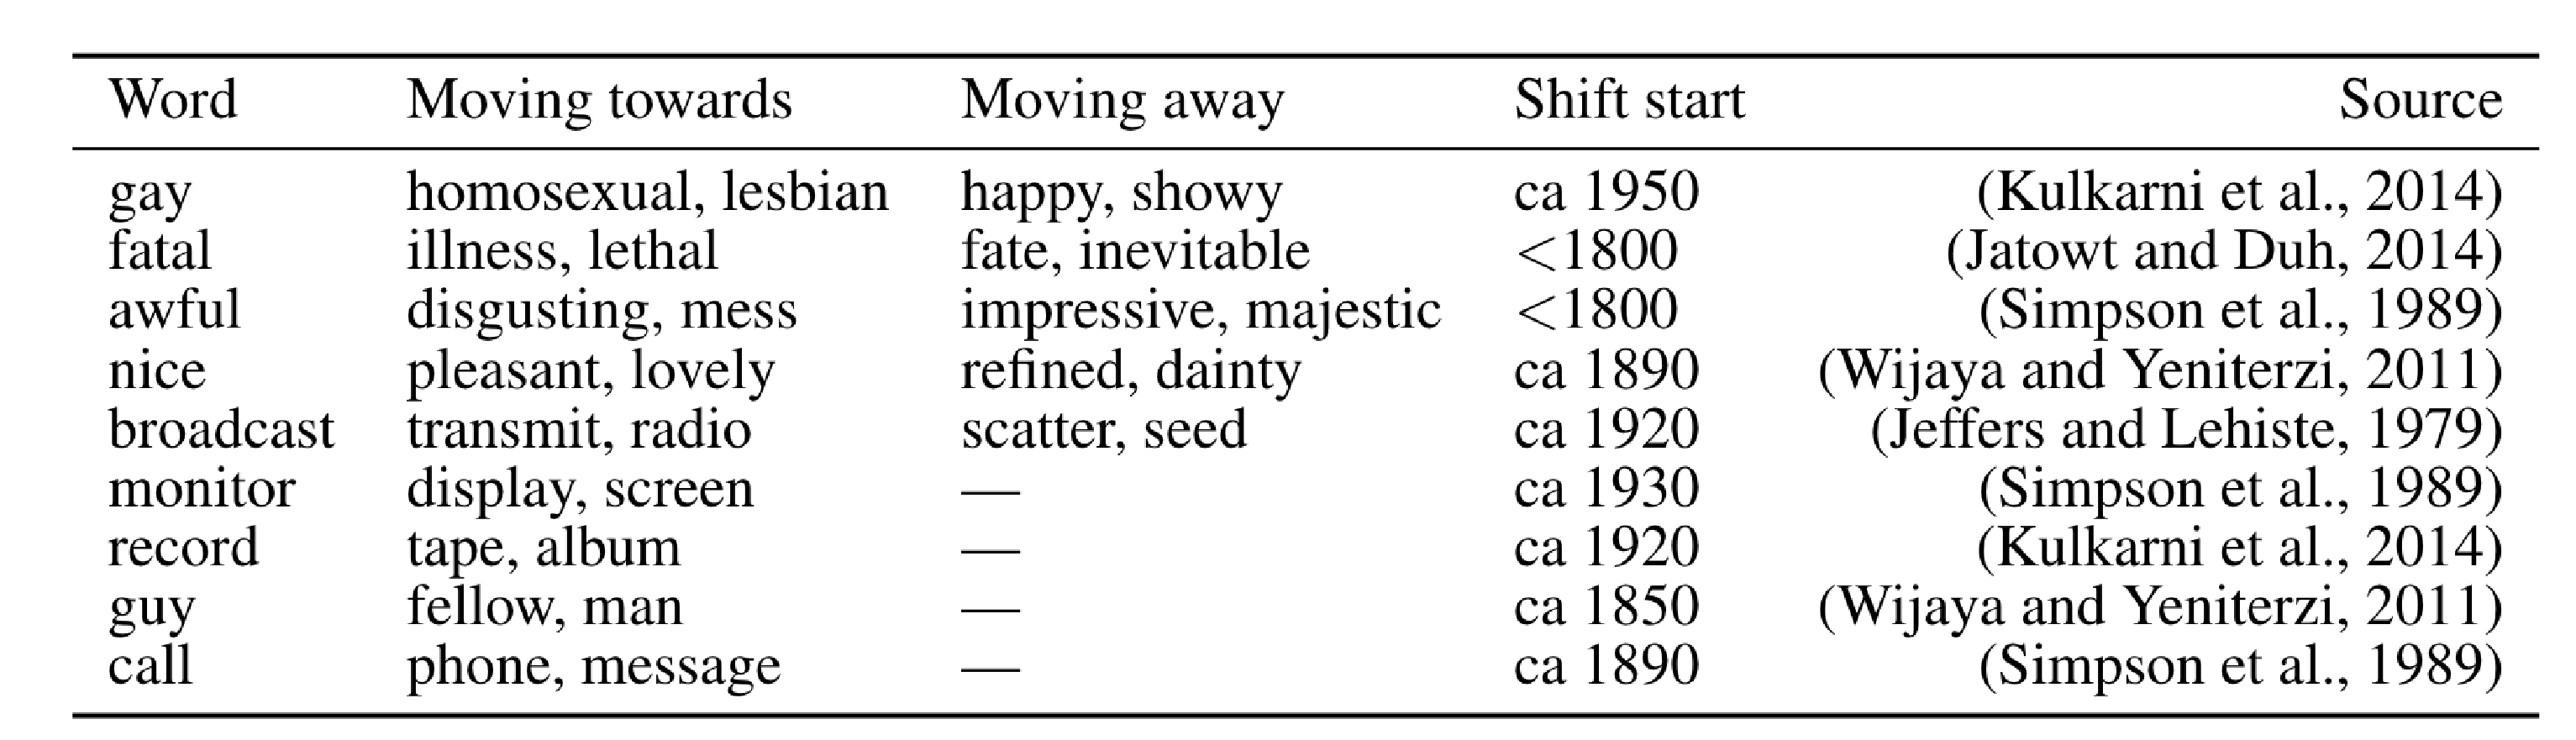
\includegraphics[scale=0.27]{figures/hamilton_known_shifts}
    \vspace*{-0.5cm}
    \caption{Known historical shifts from previous works (taken from \cite{hamilton-etal-2016-diachronic}).}
    \label{fig:hamilton-known-shifts}
\end{figure}

\textbf{Detecting Known Shifts:}
This task involves testing whether the methods can accurately capture historical shifts in word meanings that are already documented.
The goal is to determine if the methods can identify whether pairs of words have moved closer or further apart in semantic space over a specified time period.
The authors used a set of attested historical shifts as an evaluation set (\Cref{fig:hamilton-known-shifts}) to validate how well the embeddings capture these known changes.
These examples are taken from previous works on semantic change.

The results showed that all methods performed well in capturing the correct directionality of shifts, meaning they accurately identified whether word pairs became more similar or dissimilar over time.

\para{Discovering Shifts from data.}
In this task, the authors aimed to see if the methods could discover reasonable shifts in word meanings without prior knowledge of those shifts.
They examined the top-10 words that changed the most from the 1900s to the 1990s (\Cref{tab:discovering-shifts-table}) based on semantic displacement metric (\Cref{subsec:measuring-semantic-change}).
The authors categorize the words identified as having shifted meanings into three distinct categories:\\
\emph{Genuine shift:} Words that have undergone a clear and substantial change in meaning over time.
An example provided in the paper is the word `headed,' which shifted from primarily referring to the `top of a body/entity' to referring to `a direction of travel.'\\
\emph{Borderline:} These are cases where the shift is not as clear-cut, often due to global genre or discourse shifts.
These shifts might be more subtle and may not represent a complete change in meaning but rather a shift in usage within specific contexts.\\
\emph{Corpus artifacts:} These are shifts that arise not from a true change in meaning but rather from peculiarities or biases in the corpus itself.
For example, words like `special,' `cover,' and `romance' might appear to shift in meaning due to their frequent use in certain contexts like book covers or advertisements, which do not necessarily indicate a genuine semantic change.

SGNS outperformed the other methods, with 70\% of its top-10 list corresponding to genuine semantic shifts, while SVD and PPMI had lower rates of genuine shifts.

\begin{table}[tbh]
\centering
\small
\begin{tabular}{@{}llll@{}}
\toprule
\rowcolor[HTML]{FFFFFF}
\multicolumn{1}{c}{\cellcolor[HTML]{FFFFFF}}                                          & \multicolumn{3}{c}{\cellcolor[HTML]{FFFFFF}\textbf{Examples}}                                                                                                                                                                                                                               \\ \cmidrule(l){2-4}
\rowcolor[HTML]{FFFFFF}
\multicolumn{1}{c}{\multirow{-2}{*}{\cellcolor[HTML]{FFFFFF}\textbf{Semantic Shift}}} & \multicolumn{1}{c}{\cellcolor[HTML]{FFFFFF}\textbf{PPMI}}                                                    & \multicolumn{1}{c}{\cellcolor[HTML]{FFFFFF}\textbf{SVD}}                  & \multicolumn{1}{c}{\cellcolor[HTML]{FFFFFF}\textbf{SGNS}}                                        \\ \midrule
\rowcolor[HTML]{EFEFEF}
\textbf{Genuine Shift}                                                                & started                                                                                                      & \begin{tabular}[c]{@{}l@{}}headed, calls,\\ gay, actually\end{tabular}    & \begin{tabular}[c]{@{}l@{}}wanting, gay, check, starting,\\ major, actually, headed\end{tabular} \\
\cellcolor[HTML]{FFFFFF}\textbf{Borderline}                                           & \begin{tabular}[c]{@{}l@{}}know, got, would, \\ decided, think, stop, \\ remember, must, wanted\end{tabular} & male, naturally                                                           & touching                                                                                         \\
\rowcolor[HTML]{EFEFEF}
\textbf{Corpus Artifact}                                                              & -                                                                                                             & \begin{tabular}[c]{@{}l@{}}harry, wherever,\\ special, cover\end{tabular} & harry, romance                                                                                   \\ \bottomrule
\end{tabular}
\caption{The top 10 words identified by each embedding method were examined, and after reviewing the literature and analyzing their nearest neighbors,
taken from \cite{hamilton-etal-2016-diachronic}.}
\label{tab:discovering-shifts-table}
\end{table}

\subsection{Statistical Laws of Semantic Change}\label{subsec:statistical-laws-of-semantic-change}
The authors utilized diachronic embeddings to perform a large-scale cross-linguistic analysis,
revealing statistical laws that connect word frequency and polysemy to the rate of semantic change.

The authors quantified semantic change using the cosine distance metric between word embeddings across consecutive time periods, expressed as:
\begin{equation}
\Delta^{(t)}(w_i) = \text{cos-dist}(\mathbf{w}_i^{(t)}, \mathbf{w}_i^{(t+1)})
\label{eq:equation4}
\end{equation}

This equation measures how much a word’s meaning has shifted between two time periods t and t+1.
The value $\Delta^{(t)}(w_i)$ indicates the rate of semantic change for the word $w_i$.

To investigate the relationship between word frequency, polysemy, and semantic displacement, the authors performed regression analysis.
They considered data points for each word across pairs of consecutive decades.
Specifically, they analyzed how a word’s frequency and polysemy at time t correlated with its semantic displacement in the subsequent decade.

The analysis was restricted to non-stop words that appeared more than 500 times in both decades contributing to a change.
This criterion ensured that only words with sufficient co-occurrence data across years were included.

The authors employed a linear mixed model with random intercepts per word and fixed effects for frequency, polysemy, and per decade.
This model allowed them to estimate the effects of frequency and polysemy on semantic change while controlling for temporal trends and correcting for correlations between measurements on the same word across time.

\para{Law of conformity:} \emph{Frequently used words change at slower rates.}\\
The Law of Conformity states that the rates of semantic change scale with a negative power of word frequency.
This means that words that are used more frequently tend to change their meanings at a slower rate compared to less frequently used words.

This finding suggests that words with higher frequencies are more resistant to semantic shifts, confirming the Law of Conformity.
The authors demonstrated this law by presenting results using SGNS embeddings.

\para{Law of innovation:} \emph{Polysemous words change at faster rates.}\\
The Law of Innovation posits that words with higher levels of polysemy—meaning they have multiple meanings—experience higher rates of semantic change.
The authors measured a word’s polysemy by examining its neighborhood in an empirical co-occurrence network.
They constructed these networks for the top 10,000 non-stop words in each language using the Positive Pointwise Mutual Information (PPMI) measure.
In these networks, words are connected if they co-occur more often than would be expected by chance.
The polysemy of a word is then quantified by its local clustering coefficient within this network.
The clustering coefficient  $d(w_i)$  measures the proportion of a word  $w_i$’s neighbors that are also neighbors of each other.

A high clustering coefficient (and thus a low polysemy score) indicates that the words a given word co-occurs with also tend to co-occur with each other.
Conversely, polysemous words that appear in disjoint or unrelated contexts will have low clustering coefficients.

The authors found that the logarithm of the polysemy score exhibits a strong positive effect on rates of semantic change.
This finding supports the Law of Innovation by showing that words with more meanings (higher polysemy) change their meanings more rapidly.

\subsection{Takeaways}\label{subsec:takeaways4}
This paper explores how different types of word embedding models, such as PPMI, SVD, and SGNS, can be used to study diachronic shifts in word meanings.
By analyzing these aligned embeddings, the authors identify two key statistical laws of semantic change.
Law of conformity shows that high-frequency words have smaller semantic displacements over time.
They used statistical models to assess the relationship between word frequency and the rate of semantic change.
Specifically, they found that the logarithm of a word's frequency had a significant negative effect on the rates of semantic change, indicating that higher frequency words change less rapidly
The Law of Innovation is established by demonstrating that polysemous words—those with diverse meanings—tend to experience greater semantic change.
The clustering coefficient was used as a key metric for measuring polysemy within co-occurrence networks, revealing that words with lower clustering coefficients (higher polysemy) are more prone to semantic shifts.
This law highlights the dynamic nature of words with multiple meanings and their tendency to innovate in linguistic evolution.


  \balance
  \newpage
  \bibliographystyle{ACM-Reference-Format}
  \bibliography{main}
\end{document}
